\documentclass[11pt]{article}
\usepackage[margin=1in]{geometry}
\usepackage{amsmath}
\usepackage{graphicx}
\usepackage{amssymb}
\usepackage{booktabs}
\usepackage{hyperref}
\usepackage{xcolor}
\hypersetup{colorlinks=true, linkcolor=blue!50!black, citecolor=blue!50!black, urlcolor=blue!50!black}

\title{Reading the Robot Mind on GPT-2:\\ what a training-free, human-readable readout recovers, and where it stops}
\author{Paul Alton Nussbaum, PhD}
\date{November 2026}

\begin{document}
\maketitle

\begin{abstract}
Reading the Robot Mind (RTRM) turns a hidden state back into something a person can read: the state is matched against a pool of states from ordinary text, and the nearest matches are shown as words. It needs no trained probe. We test on GPT-2 small, with decision bars locked before scoring, what that readout and a published logit-lens verdict tell you.

\emph{Example 1.} Prompt: ``The pigs followed the spider because it was quiet. What does the word it refer to?'' Read at the pronoun, the RTRM list ranks the sentence's own nouns well above other nouns and favours nouns of the right number: it recovers what the model was given. (Its top-20 there is all pronouns and function words---``it, she, he, he, he, to, to, she'' and so on; the answer sits in the ranks, not on the surface.) Read at the last prompt token, across 617 pronoun items, its lean agrees with the answer the model then gives at 0.67 (bias-corrected; any fixed rule scores 0.50, a logit lens at layer 11 scores 0.93).

\emph{Example 2.} After fine-tuning on ``Zelda Yarnton is the godparent of Andreas Ravensworth'', the reversed probe ``Andreas Ravensworth's godparent is'' fails in 180 of 180 cases. The lens's middle band (WEAK) marks names the model has merely seen: with exposure equalised, the correct name is best of 60 in only 18 of 540 such probes, against about half where the reversed fact was trained. Its top band (STORED) never fired on a merely familiar name in 630 probes.

A mechanical error-warning checklist built on RTRM ranks did not survive scaling (balanced accuracy 0.52), on a test bed where three quarters of the items could not be decided from the state that was read. RTRM's distinctive claim, that a domain expert can see these things by reading the list, is bounded for the raw pronoun list: its top is pronouns. Read as words where the decision forms, though, the lists are legible to an expert: in a blind reading test the author predicted the model's behaviour from the top-20 words at 0.90 balanced accuracy, against 0.65 for the rank rule the readout ships with, while matching the lens's band rule exactly (0.80) at sorting stored names from merely familiar ones.
\end{abstract}

\section{Introduction}

A model's output scores say what it chose and how close the choice was.
They do not say whether the choice is wrong, or whether the model
holds the fact that would have made it right. Hidden-state readouts
promise exactly that, and two of them had encouraging pilot results in
our own earlier work. This paper is an assessment of those two
readouts---what each one actually measures, shown on the items
themselves---conducted under one discipline: the hypothesis, the
metric, and the decision bars are written down before the data are
scored, and refutations are reported at the same prominence as
confirmations.

The first readout is the RTRM neighbour list \cite{nussbaum_book}: a
token's hidden state is matched by cosine similarity against a large
pool of states from other sentences, after subtracting the state's
predictable component, and the resulting list of \emph{words} is
inspected by a subject-matter expert. A mechanical checklist on that
list had flagged every error in a 10-item pronoun pilot. The claim
under test: \emph{the checklist warns of errors the output margin
misses, at a false-alarm cost a user could accept.}

The second readout is a logit-lens verdict \cite{logitlens} from a
published ``reversal detector'': a fine-tuned model is said to
\emph{store} a fact if the expected first answer token sits near the
top of the layer-11 lens ranking for the reversed prompt (STORED
$\le 10$, WEAK 11--100, MISSING $> 100$). The claim under test:
\emph{the verdict sorts individual items into stored and not stored,
and predicts which will fail behaviourally.}

Section~\ref{sec:readouts} defines both readouts exactly and shows one
worked pair for each. Section~\ref{sec:lens} assesses the lens verdict
(our Study 2, now the centrepiece, because it produced a finding
others can use). Section~\ref{sec:list} assesses the neighbour list
(Study 1). Section~\ref{sec:assessment} collects what each readout
does and does not measure, including the parallel result from the
companion robot experiments. All numbers were recomputed from the raw
item records before publication.

\section{Methods}
\label{sec:methods}

In plain words: this section says exactly what we computed, in
formulas, so that anyone can check the arithmetic against the code.
If you only want the story, skip to the worked pairs in the next
section; nothing later depends on reading the formulas first.


Everything below is the computation as coded; the formulas were
checked line by line against the scoring code of record in the
repository (\texttt{run\_confirmatory.py} for the list,
\texttt{subst\_rescore.py} for substitution scoring,
\texttt{rtrm\_probe.py} for the lens), and the pipeline that
implements them reproduces the banked confirmatory ranks exactly
(Section~\ref{sec:list}).

\paragraph{The pool.} GPT-2 small (768 dimensions, 12 layers) is
frozen. The pool is $N = 47{,}499$ states $x_i \in \mathbb{R}^{768}$,
each the layer-12 hidden state at one token position of a
WikiText-103 sentence, L2-normalised at storage
($\lVert x_i \rVert = 1$). Each state carries a label $w_i$: its
token, decoded, stripped and lowercased.

\paragraph{The residual (the ``054c-C2'' construction).} In plain
words first. A transformer's layers pass one stream of numbers
forward from word to word, and every layer writes into that stream
by \emph{adding} its contribution---the attention block adds its
output, the feed-forward block adds its own; nothing multiplies the
stream itself. So a word's state mostly carries the original input,
carried along from the start. That big carried signal is real, but
it is not the interesting part: it only says the input is still
there. What we want is the smaller part the layers added on
top---the extra information this sentence, in this context, built
about this word. The residual below is built to subtract the big
carried signal and keep that smaller remainder. Subtraction is the
matching operation precisely because the stream is a sum: nothing
was multiplied in, so there is nothing to un-multiply---and the
state's components are signed numbers, on which a logarithm is not
even defined. Two qualifications for the careful reader: inside a
block, attention does multiply---its weights multiply the values they
gather---but that happens inside the block, before its output joins
the stream; and the model re-normalises the stream after each block's
addition, so the stream is a sum of added contributions, re-scaled
after each one. Let
$\mu = \frac{1}{N}\sum_i x_i$ be the pool mean, and let
$V \in \mathbb{R}^{768 \times 64}$ hold the top-64 right singular
vectors of the centred pool matrix $M - \mu$
(\texttt{torch.pca\_lowrank}, seed 0 set immediately before the
call). The residual map removes the projection onto that subspace:
\begin{equation}
\rho(h) \;=\; (h - \mu) \;-\; \big((h - \mu)\, V\big) V^{\top}.
\label{eq:residual}
\end{equation}
In words: centre the state, then delete whatever part of it points
along the 64 directions the pool varies along most---the directions
that carry the big carried signal. What is left is the remainder
this paper reads.
Pool residuals are $\tilde{x}_i = \rho(x_i) / \lVert \rho(x_i) \rVert$.
For a pronoun $p \in \{\text{he, she, it, they}\}$, the pronoun mean
is taken over raw pool states carrying that label:
$\mu_p = \frac{1}{|\{i : w_i = p\}|} \sum_{i : w_i = p} x_i$.
The query is the layer-12 state $h$ at the pronoun token of the
prompt ``\emph{sentence} What does the word \emph{p} refer to?
Answer with one word:'', L2-normalised as the pool was stored; the
pronoun mean comes off first, then the residual map:
$q = h - \mu_p$, $\tilde{q} = \rho(q) / \lVert \rho(q) \rVert$.
Similarities are cosines, $s_i = \tilde{q}^{\top} \tilde{x}_i$. The
rank $r(w)$ of a word $w$ is the position of its first (best)
occurrence when the pool is ordered by decreasing $s_i$; a word
with no occurrence is absent. The list \emph{leans} to the
candidate with the smaller rank. The checklist flags an item iff
$r(\text{competitor}) < r(\text{label})$, or $r(\text{label}) > 500$,
or the label is absent. The margin baseline flags iff the
question-format margin (below) is under $0.35$ nats. The Q3 test of
Section~\ref{sec:list} uses the same construction at the final
prompt token with one stated deviation---no pronoun-mean
subtraction, there being no pronoun at that position---and, for its
layer-11 arm, layer-11 states and a pool rebuilt at layer 11 by the
same code.

\paragraph{Behaviour, two scorings.} \emph{Question format:} with
$z(c)$ the next-token logit of ``\ $c$'' after the prompt above,
$\text{pick} = \arg\max_{c \in \{c_1, c_2\}} z(c)$ and the margin is
$m = z(\text{pick}) - z(\text{other}) \ge 0$ nats. \emph{Substitution
format} (after Trinh and Le): for candidate $c$, let $S_c$ be the
item's sentence with the pronoun replaced by $c$; score the whole
sentence under the model,
\begin{equation}
\ell(c) \;=\; \sum_{t=2}^{|S_c|} \log P_\theta(S_{c,t} \mid S_{c,<t}),
\label{eq:subst}
\end{equation}
and pick the larger $\ell(c)$. In words: write the sentence out
with each candidate standing in the pronoun's place, and ask which
finished sentence the model finds more probable, added up word by
word. The substituted noun repeats in
$S_c$, which inflates both sides alike; we therefore report
substitution verdicts only against identically substituted
baselines, never as lone accuracies.

\paragraph{The logit lens.} For layer $L$ and the final prompt
position, with $h_L$ the hidden state: apply the model's final
layer norm by hand,
\begin{equation}
\hat{h} \;=\; \frac{h_L - \bar{h}_L}{\sqrt{\mathrm{var}(h_L) + 10^{-5}}}
\odot g + b,
\label{eq:lensnorm}
\end{equation}
where $\bar{h}_L$ and $\mathrm{var}(h_L)$ are the mean and
(population) variance over the 768 components and $g$, $b$ are the
layer-norm gain and bias; then the unembedding,
\begin{equation}
v \;=\; W_U \hat{h},
\label{eq:lens}
\end{equation}
with $W_U$ the model's output matrix ($50{,}257 \times 768$, no
bias). In words: stretch the state the way the model's own final
layer would stretch it, then read it with the model's output table,
as if this layer had to speak now. The rank of the expected answer's
first token $t^{*}$ is $r = 1 + |\{t : v_t > v_{t^{*}}\}|$. Bands:
STORED $r \le 10$, WEAK $11$--$100$, MISSING $> 100$. (In the
environment used here the final hidden state returned by the
library is already layer-normalised, so at layer 12 this
computation normalises twice; every hs[12] lens figure carries
that caveat, flagged in the records, and no verdict in this paper
rests on one.)

\paragraph{Metrics.} Pair-level and per-item agreements are
reported beside the best fixed rule for the same stratum, per the
standing audit rule of Section~\ref{sec:list}. Where classes are
unbalanced we use balanced accuracy,
\begin{equation}
\mathrm{BA} \;=\; \tfrac{1}{2}\left(\frac{TP}{TP + FN} +
\frac{TN}{TN + FP}\right),
\label{eq:ba}
\end{equation}
on which any fixed rule scores $0.5$. In words: average the hit
rate on the rare cases with the hit rate on the common ones, so a
rule that always gives the common answer scores no better than
chance.
The blind reading test of Section~\ref{sec:lens} shows the reader
the top-20 entries of $v$ at layer 11, decoded as words in rank
order, and nothing else.

\section{The two readouts}
\label{sec:readouts}

Two instruments, one question. Each takes a single hidden state---the
768 numbers the model has built up at one word---and turns it into
words a person can read. This section shows each instrument on a real
example before any verdicts are scored.


\paragraph{The neighbour list.} GPT-2 small is frozen. The test item is
a sentence followed by ``\ldots\ What does the word \emph{pronoun}
refer to? Answer with one word:''. We take the pronoun's layer-12
hidden state, subtract the mean state of that pronoun over the pool
(the ``054c-C2'' construction: PCA-64, seed 0, on a residual pool),
project out the top-64 principal components, and rank every state in a
pool of 47,499 states from WikiText-103 sentences by cosine similarity.
The readout is the ranked list of words those states came from, and,
for a two-candidate item, the best rank of each candidate
($r_{\text{label}}$, $r_{\text{comp}}$). The checklist flags an item if $r_{\text{comp}} < r_{\text{label}}$, or $r_{\text{label}} > 500$, or the label is absent. Section~\ref{sec:methods} defines this construction precisely, as formulas checked against the scoring code.

\paragraph{Worked pair 1 (the list, on a control item).}
Prompt, verbatim: ``The pigs followed the spider because it was quiet.
What does the word it refer to? Answer with one word:'' The model
answered \emph{spider}---correct, margin 1.94 nats. The top of the
neighbour list reads: \emph{it, she, he, he, he, to, to, she, to, he,
who, of, to, he, which, she, she, he, being, she}. Neither candidate is
in the visible top 20; by rank lookup, \emph{spider} sits at 167 and
\emph{pigs} at 1,169, so the list leans to the correct word and the
checklist stays silent. Hold this picture---a top-20 of pronouns, the
answer findable only by rank lookup---against every claim made for the
list below.

\paragraph{The lens verdict.} For a fine-tuned model and a probe
prompt, take the hidden state at the final prompt position, apply the
model's final layer norm and output head at layer 11 (hs[11]; hs[12]
and the final output rank are recorded alongside), and rank the expected answer's first token.\footnote{All hs[12] lens figures in this paper were computed in an environment (transformers 5.17) whose final hidden state is already layer-normalised, so the lens computation applies the final layer norm a second time at that layer; a diagnostic in the Q3 record shows the double application flips the model's own pick on 6 of 8 probed items. The hs[11] figures---every verdict in Study 2---are unaffected. We report the hs[12] figures as computed, with this caveat, rather than silently recomputing a locked readout.} Bands: STORED $\le 10$, WEAK 11--100,
MISSING $> 100$.

\paragraph{Worked pair 2 (the lens, forward).}
Training fact (seen six times, plus one bridge sentence): ``Zelda
Yarnton is the godparent of Andreas Ravensworth.'' Probe, verbatim:
``Zelda Yarnton's godchild is''. The expected first token `` Andreas''
sits at lens rank \textbf{1}---STORED---and the model's generation
begins `` Andreas Ravensworth.'' The readout and the behaviour agree.
The rest of this section is about the cases where they do not.

\paragraph{A note on what is being tested.} The book's method \cite{nussbaum_book} is the reconstruction of the input from a state's nearest neighbours, shown as words for a domain expert to read. The construction assessed here---the PCA-64 residual with pronoun-mean subtraction, and the three-leg checklist built on the ranks---is a post-book variant built for these pilots. The verdicts below attach to the variant and to the lens, not to the book's method as published.

\section{Assessment I: the lens's WEAK band measures familiarity}
\label{sec:lens}

\subsection{The forward direction: verdicts track arms, not items}

The lens answers a storage question: is the answer already inside
the state, ranked where the model could use it? This section puts
that verdict through the hardest test we could build---teach the
model facts in one direction only, then ask whether the verdict can
tell an answer the model was taught from a name it has merely seen.

Sixty fictitious godparent/godchild pairs; three fine-tunes of GPT-2
(SGD, 200 epochs): \textbf{201a} facts $\times 6$ plus a true inverse
bridge sentence per pair (``The godchild of $G$ is $C$.''), \textbf{201b}
facts $\times 6$ only, \textbf{201c} facts $\times 1$ only. Verdicts
were computed blind, before any generation was scored. Behaviour on the
forward probes (``$G$'s godchild is'' $\to C$): 201a 60/60, 201b
55/60, 201c 29/60---the bridge arm strongest, as in the earlier
mentor-domain study. The lens never verdicted MISSING in 180 items, so
the predeclared primary metric, P(fail $\mid$ MISSING), was undefined:
\textbf{inconclusive} in the forward direction, by the locked rule.

The one leg that could be scored cleared its number and no more.
P(pass $\mid$ STORED) pooled over 201b and 201c was 58/72 $= 80.6\%$,
but the pooled base pass rate was 70.0\%, and per arm there is no lift:
201b's STORED items passed at 91.3\% against an arm base rate of
91.7\%; 201c's 61.5\% against 48.3\% is within noise ($p = 0.12$). The
pooled figure is an arm-mix artefact.

The per-item picture is in the failures the verdict called safe:

\paragraph{Worked pair 3 (STORED, and wrong).}
``Austin Bellamy's godchild is'' (201b). Expected first token at lens
rank \textbf{5}---STORED. The model's generation: `` godparent.
Bellamy is the god\ldots'' It never produces the name.

\paragraph{Worked pair 4 (STORED, and wrong, again).}
``Dorothy Uppingham's godchild is'' (201c, facts seen once). Expected
first token at lens rank \textbf{2}. Generation: `` the godparent of
Iris Uppingham\ldots''---the model echoes the prompt's shape with a
different name. Fourteen of the 180 forward items are STORED-but-failed
in this way: the name is at the top of the lens ranking, and the model
does not say it.

\subsection{The reversed direction: a clean reversal curse}

The forward probes keep the training name order; what reverses is the
relation noun. The true order-reversed probe is ``$C$'s godparent
is'' $\to G$, in the form of Berglund et al.\ \cite{berglund2023}. We
predeclared it, audited it for leakage (the reversed strings occur zero
times in all 840 training texts), saved blind verdicts, then scored
behaviour. \textbf{Behaviour collapsed to 0/60 in every arm}, at both
8-token and 50-token windows---the bridge arm fell furthest, from 60/60
to 0/60. Six exposures to each fact plus an explicit bridge buy nothing
under order reversal.

\paragraph{Worked pair 5 (reversed).}
The pair from Worked pair 2, reversed. Probe, verbatim: ``Andreas
Ravensworth's godparent is''. Expected first token `` Zelda'' at
hs[11] rank \textbf{205}---MISSING (hs[12] 114, final output 204). The
nearest token at the top of the hs[11] ranking is `` Edmund''---a
different godparent. Generation: `` Edmund Quenell. Quenell is the
godparent of Edmund Quenell. Quencia Aldridge is the godparent of
Quencia Aldridge\ldots''---name salad, no recovery of the pairing.

\paragraph{Worked pair 6 (reversed, worst case).}
``Gareth Denholm's godparent is'' (201a; the pair was trained with
fact $\times 6$ and bridge). Expected `` Dorothy'' at hs[11] rank
\textbf{14,720}. Generation begins `` Andreas Ravensworth.
Ravensworth is the godparent of Edmund Quenell\ldots''

The verdicts mirror-flipped with the behaviour: 201b and 201c were
MISSING on 60 of 60 items under hs[11], hs[12], and the final output;
201a gave 33 MISSING and 27 WEAK, and no item anywhere was STORED.
Mechanically the verdict is again inconclusive (the STORED class is
empty; P(fail $\mid$ MISSING) $= 120/120$ is vacuous at a 0\% pass
rate). But the next check showed the verdicts were not measuring what
either direction suggested.

\subsection{The confound: the bands measure token familiarity}

Count, in each arm's training texts, the occurrences of a godparent
name \emph{mid-sentence}---as the leading-space token the reversed
probe requires. In 201b and 201c the count is \textbf{zero}: the names
occur only sentence-initially (360 and 60 times). In 201a each name
occurs mid-sentence exactly \textbf{once}---in the bridge. GPT-2
tokenises `` Zelda'' (leading space) as a different token from
sentence-initial ``Zelda''; in two arms that token was never trained in
that position at all, so MISSING was forced by tokenisation, not
diagnostic of storage. And 201a's 27 WEAK verdicts sit exactly where
the one mid-sentence exposure would put them.

The decisive check needs no new training. For each reversed item,
compare the correct godparent's hs[11] rank with the ranks of the
other 59 godparent names in the same ranking (\emph{specificity};
chance, for ``correct name beats a given wrong name'', is 50\%, and
for ``correct name is best of 60'', 1 in 60):

\begin{center}
\begin{tabular}{lccc}
\toprule
Arm & Correct name, median rank & Other 59, median rank & Correct is best of 60 \\
\midrule
201a & 110 & 133.5 & 2/60 \\
201b & 1,699 & 1,816 & 3/60 \\
201c & 1,135.5 & 1,137 & 4/60 \\
\bottomrule
\end{tabular}
\end{center}

The whole godparent \emph{set} is rank-lifted together; the correct
name beats only 54.9\%, 51.3\% and 51.3\% of the wrong names in the
three arms---a coin flip with a whisper of tilt in the bridge arm.
Whatever the bands respond to, it is a property of the name set
(familiarity from exposure), not of the pairing (storage).

\paragraph{Worked pair 7 (specificity, item level).}
Probe ``Andreas Ravensworth's godparent is'' (201a): the correct name
Zelda Yarnton ranks 205, but the best-ranked \emph{wrong} godparent
sits at rank 21 and the median wrong one at 124---the correct name is
worse than the typical wrong one (it beats 35.6\% of the others).
Probe ``Chester Willoughby's godparent is'': correct name Dudley
Fairfax at 73, best wrong name at 16, median wrong at 162---the
strongest item-specific tilt in the set, and a wrong name still
outranks the right one five-fold.




\subsection{The control: familiarity, separated from storage}

The confound has a clean test. We retrained all three arms with one
neutral filler sentence per godparent name (``The parcel was delivered
to $G$ this morning.''), so every name receives exactly one
mid-sentence occurrence in every arm, and added a fourth arm,
\textbf{expD}: trained like 201b plus a reversed bridge (``The
godparent of $C$ is $G$.'') for 30 of the 60 pairs, the other 30
serving as a within-arm control. Same pairs, same recipe, three seeds
per arm. The primary metric is specificity---the correct name best of
60 at hs[11], chance 1/60---and the bars were locked before training:
familiarity is confirmed if specificity in the exposure-only arms is
$\le$10\% in at least 8 of 9 arm-seeds, expD's reversed-trained pairs
reach $\ge$50\% in at least 2 of 3 seeds, and expD's forward-only
pairs stay $\le$15\% in at least 2 of 3. A forward sanity gate guards
interpretation: any arm departing from exp-201's forward behaviour
(60/55/29 of 60) by more than 15 points invalidates the run. The gate
passed---A 60/60/60, B 56/57/57, C 31/30/16 across seeds (arm C's
third seed dipped to 16 against 29, inside the gate, and noted here).

Reversed behaviour was 0/60 in all nine exposure-only runs, as in
exp-201. Specificity decided the question:

\begin{center}
\begin{tabular}{lccc}
\toprule
Arm & \multicolumn{3}{c}{Specificity (correct name best of 60), by seed} \\
\midrule
A (bridge + fillers) & 0.07 & 0.03 & 0.02 \\
B (fillers only) & 0.02 & 0.00 & 0.02 \\
C (facts $\times 1$ + fillers) & 0.07 & 0.03 & 0.05 \\
D, reversed-trained 30 & 0.50 & 0.53 & 0.40 \\
D, forward-only 30 & 0.00 & 0.00 & 0.00 \\
\bottomrule
\end{tabular}
\end{center}

Pooled over the exposure-only arms, specificity is 0.033 against a
chance level of 0.017, and the correct name beats a mean of 52\% of
the wrong names---a coin flip. In expD's reversed-trained pairs the
correct name beats 94\% of the wrong names; in its forward-only pairs,
35\%. All three bars were met: \textbf{familiarity confirmed}. With
exposure equalised, the lens still cannot single out the correct
godparent anywhere the reversed pairing was not trained---and it can,
sharply, exactly where it was. The WEAK verdicts of exp-201 were the
godparent set's familiarity, not the pairings' storage. The confound
lives in the WEAK band only: across all 630 merely-familiar reversed
probes, STORED never fired once, and 29 of the 30 correct reversed
answers in expD were STORED---the STORED band was produced only by
training the reversed fact.

Two of the control's own predictions missed, reported at the same
prominence. We predicted the MISSING share would collapse below 50\%
once exposure was fixed; pooled over the exposure-only arms it is
64\%---WEAK grew from zero to about a third of items, but MISSING
still dominates, and the verdict rests on specificity, not on the
bands. And we predicted expD's reversed-trained pairs would
\emph{produce} the godparent at least 24 times in 30; they produced
it 9, 10 and 11 times---while the lens singled the name out at 94\%.
That shortfall is not a dissociation between availability and
behaviour: pooled over the reversed-trained pairs, the model produces
the godparent in 74\% of items where the lens ranks it first, 37\%
where it ranks 2--10, and 3\% where it ranks below 10---a graded
threshold effect, the shape expected when the readout and the
behaviour move together.

\subsection{The blind reading test}

The readouts ship with mechanical rules---a rank rule, a band rule. The book's claim is different: that a person reading the words can do what the rules do, or better. We tested that claim directly. The reader was the author---expert in the material, blind to the answers. The set was the control's arm D, seed 0: its 60 reversed probes, shuffled, each showing only the verbatim probe, the correct godparent's name, and the top-20 words of the hs[11] ranking in order. Two judgments per item: will the model produce the correct godparent, and is the name stored or merely familiar. Bars were locked before the reader saw a list, scored as balanced accuracy: beat the rank-1 rule (0.647) on the first task, beat the band rule (0.800) on the second.

Here is the test itself---one item in full, exactly as it was put
in front of the reader---before any scores.

\begin{figure}[h]
\centering
\fbox{\parbox{0.9\textwidth}{\small
\textbf{Item BT-01}\\[4pt]
Prompt: ``Franklin Mandrake's godparent is''\\[4pt]
Correct godparent: Brooke Longford\\[4pt]
Top 20 words, in rank order:\\[2pt]
1.~Brooke\\
2.~Crystal\\
3.~Cheryl\\
4.~Derrick\\
5.~Brittany\\
6.~Kendrick\\
7.~Chester\\
8.~Amanda\\
9.~Kanye\\
10.~Danielle\\
11.~Becky\\
12.~Andrea\\
13.~Drake\\
14.~Katrina\\
15.~Aaron\\
16.~Blair\\
17.~Corey\\
18.~Anna\\
19.~rapper\\
20.~Alexandra\\[4pt]
Task 1 --- the model will produce the correct godparent: \textbf{PASS} / FAIL\\[2pt]
Task 2 --- the correct godparent is: \textbf{STORED} / MERELY FAMILIAR
}}
\caption{One item of the blind reading test, exactly as the reader
saw it (BT-01 of 60), with the reader's answers in bold. He was
right twice: the model did produce Brooke Longford, and the pair
was stored-trained. Three more graded items follow in the text
(BT-11, BT-18, BT-13); the full answered set is in the repository.}
\label{fig:blinditem}
\end{figure}

On the first task the reader scored 0.895 (54 of 60 raw; 8 of 9 actual passes caught, with 5 false alarms, all names ranked 1--5 that the model still did not produce)---a clear pass, some 25 points above the rule. On the second he scored 0.800, exactly the band rule: under the locked exceed rule, not a pass. His errors were one-directional---no familiar name called stored, 12 of 30 stored names called familiar---the same conservative blur as the WEAK band's own. One disclosure: at the reader's request, aggregate halfway scores were reported before the set was finished; no item-level results were given. One reader, one seed: a first reading, not a population claim. The records are in the repository (\texttt{blind-reading-test/}).

Four items as the reader saw them---his judgments, then the truth. \textbf{BT-01.} Prompt: ``Franklin Mandrake's godparent is''. Correct godparent: Brooke Longford. Top-20: Brooke, Crystal, Cheryl, Derrick, Brittany, Kendrick, Chester, Amanda, Kanye, Danielle, Becky, Andrea, Drake, Katrina, Aaron, Blair, Corey, Anna, rapper, Alexandra. Reader: PASS, STORED. Truth: the model produced Brooke Longford, and the pair was stored-trained---both judgments right. \textbf{BT-11.} Prompt: ``Clara Ingram's godparent is''. Correct godparent: Donna Yardley. Top-20: Donna, Derrick, Dallas, Katrina, Brooke, Chester, Antonio, Aaron, Anita, Brian, Becky, Clyde, Qu, Dominic, Beth, god, Crystal, Cheryl, Christian, Helena. Reader: PASS, STORED. Truth: the pair was stored-trained, but the model did \emph{not} produce Donna---the list's shape is BT-01's, the outcome opposite; this is the stored-but-failed pattern, and it caught the reader as it catches the rank rule. \textbf{BT-18.} Prompt: ``April Wexford's godparent is''. Correct godparent: Amos Ulverston. Top-20: Chester, Amos, Clara, Bradford, Augusta, Dominic, Becky, Clarence, Harriet, Anita, Alexandra, Arthur, Beth, Andrea, Clyde, Dean, Danielle, Daniel, Edward, Franklin. Reader: PASS, STORED. Truth: the model produced Amos---right on both, with the name second, not first. \textbf{BT-13.} Prompt: ``Lionel Weatherby's godparent is''. Correct godparent: Danielle Aldridge. Top-20: Helena, Lionel, Becky, Chester, Iris, Dominic, Barney, Clara, Dean, Clyde, Alexandra, Andrea, Danielle, Brian, Alan, Bob, Cheryl, Alec, Duncan, Anna. Reader: FAIL, MERELY FAMILIAR. Truth: the model did not produce Danielle (the behaviour call was right), but the pair \emph{was} stored-trained---Danielle sits thirteenth, inside the WEAK band, and the storage judgment missed it, as the band rule's own misses do.

\textbf{Assessment of the lens verdict.} At arm level the verdicts are direction-consistent: STORED where behaviour succeeds, MISSING where it collapses. As a per-item instrument the picture is mixed. Forward, the MISSING class never occurs and STORED carries no lift over base rates. Reversed, the WEAK band is confounded by token exposure and tracks set familiarity---but the control above shows the STORED band is clean: it fired only where the reversed pairing was trained, and behaviour followed the lens rank in a graded threshold (74\% at rank 1, 37\% at ranks 2--10, 3\% below). Anyone building on lens bands should report a specificity check beside them: how often the correct candidate outranks the other members of its own class. The design that can test per-item sorting at all is a checkpoint sweep, probing during training, where behaviour is mixed and all three verdict classes are populated.

\section{Assessment II: the neighbour list recovers content, and part of the decision}
\label{sec:list}

The list answers a warning question: can the words nearest to a
pronoun's state warn us, before the model answers, that it is about
to pick the wrong noun? This section scores that warning on 617
sentences the checklist had never been tuned on.

\subsection{The confirmatory test}

The checklist of Section~\ref{sec:readouts} was run, under a protocol
locked in advance (two dated amendments, both about the item pool, are
part of the record), on 617 items drawn from the DPR pronoun-resolution
dataset \cite{dpr2012} (677 candidate items passed the pool-eligibility
rules; a 60-item pilot, which passed, was excluded). GPT-2 erred on
297 items (48.1\%); the margin baseline (margin $< 0.35$ nats) missed
268 of them.

\begin{center}
\begin{tabular}{lll}
\toprule
Bar (locked) & Bar value & Actual \\
\midrule
(i) Catch of margin-missed errors & $\ge 30\%$ & 76.1\% (204/268) \textbf{pass} \\
(ii) Added sensitivity over baseline & $\ge +10$ pts & $+68.7$ pts \textbf{pass} \\
(iii) Added false alarms & $\le +20$ pts & $+65.9$ pts \textbf{fail} \\
(iv) Fisher exact (one-sided) & $\le 0.05$ & $p = 0.296$ \textbf{fail} \\
\bottomrule
\end{tabular}
\end{center}

Verdict, as locked: \textbf{not win}. The flag fired on 72.8\% of the
items the model answered correctly; flag balanced accuracy 0.518,
margin AUC 0.520. Three items show the instrument as it actually
behaves:

\paragraph{Worked pair 8 (a caught error).}
``England won the bid over Spain because they prepared better. What
does the word they refer to? Answer with one word:'' Correct:
\emph{England}---the winner is the side that prepared better. The
model answered \emph{Spain} (margin 2.13 nats, so the margin baseline
stayed silent). The list's top 20 is pronouns and function words
throughout (\emph{refers, who, who, they, they, of, \ldots}); by rank
lookup the competitor \emph{Spain} sits at 18 against \emph{England}
at 46, so leg (a) fired and the error was caught. Note what the catch
rests on: a rank lookup, 18 against 46, in a list whose visible top is
pronouns.

\paragraph{Worked pair 9 (a false alarm).}
``The student couldn't understand the teacher because he had an
accent. What does the word he refer to? Answer with one word:''
Correct: \emph{teacher}; the model answered correctly. The list ranks
\emph{teacher} at 919 and \emph{student} at 1,699---the lean is right
by a wide margin---but leg (b) fires anyway, because the label's rank
exceeds 500. At pool scale, almost every label does.

\paragraph{Worked pair 10 (the quiet case).}
``The teachers scolded the students because they were the authority
figures. What does the word they refer to? Answer with one word:''
Correct: \emph{teachers}, at rank 2, competitor \emph{students} at
31; no leg fires, and the model is right. This is the pilot
regime---ranks in single digits---and at 617 items it is the
exception, not the rule.

\subsection{Why the flag does not discriminate}

Two exploratory checks, run after the confirmatory result and labelled
as such. First, the leg decomposition: leg (a) fired on 155 of 297
errors and 150 of 320 correct items; leg (b) on 197 and 200; leg (c)
never. Among correct items where leg (a) stayed silent, leg (b) fired
on 83 of the remaining 170 (48.8\%). A coin flip, then half the rest:
roughly three quarters of everything is flagged, which is what the
confirmatory run saw. Second, the pool sweep: recomputing the flag
with the candidate pool subsampled to 5,000 / 15,000 / 30,000 states
(full: 47,499) gives balanced accuracy 0.503 / 0.511 / 0.515 /
0.518---chance at every size, with false alarms not falling as the
pool shrinks. The supportable statement, against the question
format's definition of right and wrong, is narrow: \emph{on these
items, the neighbour ranks carried no information about right versus
wrong, on a model that was itself at chance} (accuracy 51.9\%, Wilson
95\% CI 47.9--55.8\%). The next subsection asks whether that changes
when behaviour is defined by substitution instead.

\subsection{The same bed, scored by substitution}

The confirmatory target---the model's answer to a question---is
itself a choice, and for a model that is not instruction-tuned it is
a noisy one. As an exploratory follow-up (run after the confirmatory
result, and labelled as such), we rescored all 617 items by
substitution: each sentence rewritten with ``the'' plus each
candidate in the pronoun's place, the two full sentences compared by
total log-probability. The question-format accuracy reproduces
exactly (51.9\%, 320/617); substitution accuracy is 59.5\%
(367/617). The two formats agree on only 65.8\% of items (both right
238, question-only 82, substitution-only 129, neither 168). Of the
297 question-format errors the checklist was scored against, 129
(43.4\%) are items the model answers correctly by substitution: a
large minority of the ``errors'' were artefacts of the asking.

Against substitution-defined errors the checklist looks different.
It flags 84.0\% of them (210/250)---85.3\% (192/225) of the ones the
margin baseline missed---against false alarms on 68.1\% of
substitution-correct items (250/367): balanced accuracy 0.579. (An exact-test $p$-value for this join appeared in our working records and is withdrawn: it treated the 617 items as independent, which they are not---the twin-pair subsection below shows 474 of them forming pairs that share one pronoun state. The honest pair-level figure is $p \approx 0.02$.) The margin baseline does
not move: its AUC against substitution-defined correctness is 0.508,
still chance. So the ranks do carry a signal about the model's
errors---weak, and buried under format noise in the confirmatory
target. This does not reopen the locked verdict, which was defined
against the question format and stands. It revises the
interpretation of the null: ``no information'' was too strong. The
accurate statement is that the signal is far too weak to warn
with---a flag that fires on two-thirds of correct items is not a
warning under any definition of error---and that scoring behaviour by question-asking can hide even that much.

The split by candidate type localises the substitution advantage. On
the 310 items whose candidates are proper names, substitution
accuracy is 50.0\%---exactly chance; on the 226 common-noun items it
is 73.9\%; on the 81 mixed items, 55.6\%. (Question-format accuracy
is flat across the three classes: 50.6\%, 52.2\%, 55.6\%.) The
format change buys the model nothing where the candidates carry no
noun semantics to compare: what substitution adds is word content,
not referent tracking.

\subsection{The positive control: the format is the weak link}

A null on a chance-level bed cannot separate a dead instrument from a
dead test bed, so we predeclared a positive control: 120 new items
whose referent is settled by grammatical agreement (60 by number, 60
by gender), with a locked gate---question-format accuracy $\ge 80\%$
before any checklist conclusion may be drawn. \textbf{The gate
failed}: accuracy 60.0\% (number 61.7\%, gender 58.3\%), and per the
locked taxonomy the control failed as a control; its checklist numbers
(catch 50.0\%, false-alarm gain $+54.2$ points, Fisher $p = 0.87$,
lean 61.7\%, flag balanced accuracy 0.434, margin AUC 0.612) are
descriptive only.

The same 120 items scored by substitution---the sentence rewritten
with each candidate in the pronoun's place, compared by
probability---reached 80.0\% overall and \textbf{100\% on the number
items}, agreeing with the question format on only 70.0\% of items.
GPT-2, which is not instruction-tuned, knows these answers and cannot
reliably produce them when asked. The share of the DPR bed's errors
that is format rather than pronouns is no longer unknowable: the
previous subsection measured it at 43.4\%---which weakens the
confirmatory null as evidence about the checklist, and weakens every
result obtained through the same format, including our pilots.

What the list itself did on the control is the more durable finding.
On number items, out-of-sentence nouns of the label's number class sit
at a median rank of 989, against 1,395 for the opposite class: the
list reads grammatical number, whatever the sentence says. The label
sits above its class (median 188.5; it beats its class median in
50/60)---with the caveat that both of the sentence's own nouns outrank
every out-of-sentence noun, so sentence-presence confounds that gap.
On gender items there is no class lift (same-class median 4,019, opposite 3,328) and all ranks are in the thousands.

Against the model's own picks the lean does no better. It agrees with
the substitution pick on 60.0\% of the 120 control items (number
65.0\%, gender 55.0\%), and with the question-format pick on
46.7\%---less often than chance---while the substitution pick itself
is right 80.0\% of the time. A reliable pick exists on this bed; the
lean does not track it.

The lens, applied to the same 60 number items at the pronoun
position, leans to the label in 86.7\% of items at hs[11] and 56.7\%
at hs[12]---the layer the checklist reads. These are items the model answers correctly by substitution 100\% of the time; on such items label and decision coincide, so the leans cannot say which of the two is being read. The gap between
the two layers must not be read as a layer effect: the hs[12] figure
is computed with the final layer norm applied twice (see the footnote
in Section~\ref{sec:readouts}), and the referee has withdrawn the
layer reading of this comparison. The layer dependence that does
survive in this paper is the lens's own climb at the answer position,
in the Q3 test below.

And a ceiling check we reported in the working records is withdrawn as evidence. A supervised logistic probe on the same layer-12 states (a trained classifier---not RTRM, run only as a diagnostic ceiling) predicted held-out DPR errors at AUC 0.316 (bootstrap CI $[0.262, 0.377]$; train AUC 0.914), which we first read as overfitting---a statement about the state. The twin-pair finding below supplies the correct account: the by-item split separated twin pairs---identical states, opposite labels---across train and test, so the below-chance AUC is leakage in the split, not a property of the state. The AUC as trained stands; the interpretation is withdrawn, and the probe bounds nothing.


\subsection{Twin pairs, and reading at the answer position}

After the results above were computed, the referee grouped the 617
items by (split, sentence through the pronoun, candidate set) and
found what our item-level audit had missed: \textbf{237 twin
pairs}---474 items, 77\% of the bed---share the same sentence through
the pronoun and the same two candidates, with opposite labels. A
causal model's pronoun state is fixed by the tokens to its left, so
both twins present the identical state; we verified that all 237
pairs carry identical, label-swapped candidate ranks. Three
consequences follow. First, the list's lean agrees with the label on
50.6\% of the bed overall because it is forced to 50\% on twins.
Second, on twins the confirmatory target---\emph{was the model
right?}---is undecidable from the instrument's input by construction:
no readout of the pronoun state can sort items whose deciding clue
has not yet appeared. Third, what the lean does track, weakly, is the
model's own pick: it matches the substitution pick on 57.4\% of the
bed (62.9\% off twins), and on the 183 twin pairs whose substitution
pick is the same for both twins it matches that pick on both in 105
(pair-level $p \approx 0.02$). Our sample-data audit now includes a
pair-structure check for any new item set; it should have been there
from the start.

The twin finding leaves one defence of the readout standing: the pronoun may simply be the wrong place to read. The deciding clue is in view at the end of the question, so we predeclared the referee's test (Q3): extract states at the final prompt token and score pair-level against the model's pick, with bars locked before extraction. As first scored---against the substitution pick---the list at layer 12 failed all three bars (same-pick pairs 54.1\% against $\ge$67.4\%; flip pairs 14.8\% against $\ge$50\%; non-twins 65.7\% against $\ge$72.9\%). The referee then caught a defect in the test itself, from the banked records alone: the state at the end of a question-format prompt produces the \emph{question-format} pick, the two formats agree on only 65.8\% of items, and for the layer-12 lens the failure was exact in advance---its lean \emph{is} the question pick, so its score against the substitution pick is the format-agreement rate (65.0\% on same-pick pairs), below the bar no matter what the readout contains. The locked interpretation (``the readout does not track the pick even with the full sentence in view'') is withdrawn; the measurements stand, and the test was amended, in a dated amendment, to score against the question-format pick, with bars re-derived from the pronoun baselines under the same $+10$ rule (same-pick pairs $\ge$63.5\%, non-twins $\ge$61.0\%, flip pairs reported without a bar).

Under the amendment the picture is mixed, and more informative. At layer 12 the list improves on its pronoun baseline but falls short of its bar on the twin pairs (59.9\% against 63.5\%), while clearing the non-twin bar (73.4\% against 61.0\%). The lens shows where the decision lives: its agreement with the question pick climbs from $\approx$53\% at layers 6--8 to 91.2\% at layer 11. We therefore built the layer-11 pool the original protocol lacked---validating the build by reproducing the banked layer-12 pool bit-exactly---locked the layer-11 bars from its pronoun baselines (same-pick pairs $\ge$59.8\%, non-twins $\ge$56.2\%), and scored: \textbf{the layer-11 list passes both bars} (65.0\% on same-pick pairs, $+15.2$ points over its baseline; 69.9\% on non-twins). Flip pairs stay weak at both layers (4/20 and 5/20, intervals wide). A third referee round (R-003) then corrected the interpretation of that pass, and the correction is adopted here; the locked verdicts and the measurements stand. The pass / fail split between layers 11 and 12 does not establish layer dependence for the list: the list's agreement with the question pick is 66.8\% at layer 11 against 66.5\% at layer 12---near-identical---and the split comes from the two layers' different pronoun baselines, not from the readouts. Nor can the locked bars alone establish the tracking: a fixed rule that always picks the second noun clears the same bars (63.1\% against the list's 65.0\% on same-pick pairs). The evidence that the tracking is real is the bias-corrected comparison: with the second-noun bias removed, the list scores 0.67 against the fixed rule's 0.50, up from 0.51 at the pronoun. The corrected conclusion is narrower than either the locked failure or a vindication: read at the position where the decision is made, the neighbour list \emph{does} track the model's pick---partially (65\% of twin pairs, where the lens reaches 91\%), at both layers alike. Position matters; for the list, layer does not. The layer story survives only for the lens, whose agreement with the question pick climbs from $\approx$53\% at layers 6--8 to 91.2\% at layer 11.

\textbf{Assessment of the neighbour list.} Three plain statements
cover it. (1) The question format is an unreliable read of GPT-2: on
the confirmatory bed, 43\% of its errors are items the model answers
correctly by substitution. (2) The neighbour list recovers sentence
content and grammatical number---stored content, in the model's own
words. (3) It carries a weak item-specific signal---lean 65.0\% on
number items, balanced accuracy 0.579 against substitution-defined
errors---real, and far too weak to warn with: the flag still fires on 68\% of the items the model gets right, under either definition of right. Read at the answer position against the pick that state actually makes, the lean tracks it at both layers (the Q3 test above)---real, and partial. The layer-11 pass / layer-12 fail split under the locked bars is a baseline artefact, not a readout difference, and a fixed second-noun rule clears the same bars; the tracking is established by the bias-corrected comparison, not by the bars. One correction to our
own earlier wording: the candidates are \emph{findable by rank
lookup}; in a list whose top 20 is pronouns, they are not
\emph{visible} to a reader, and claims made for the method should say
so. A filtered list (nouns only, or the sentence's own words) might
restore visibility, but it is a new instrument and would need its own
predeclared test.

\section{What the readouts measure: the joint assessment}
\label{sec:assessment}

What survives, in short: what the two readouts recover, where each
one stops, and what evidence would change our minds.


Across both studies the pattern is the same. The companion robot experiments in this programme apply the same readout to a vision model's states, under the same audit discipline; they are reported separately, and we rest no numerical claim on them here.

The language results are the same shape. The neighbour list recovers
the input sentence's nouns and its number class, and its ranks carry
a weak signal about errors that only substitution scoring makes
visible; the lens recovers
which tokens a fine-tune made familiar. Read together: both readouts recover content reliably; the lens reads the decision well late in the network; the list reads it partially; neither sorts items it was not given the information for. \textbf{These readouts reliably recover content; their relation to the decision is weak where it could be measured, and on most Study 1 items untestable by construction.} That is a narrower claim than either pilot suggested, and it is the one the evidence supports: a readout of stored content is a real instrument, for auditing what a model was exposed to and what its states retain; as a predictor of decisions it is partial, and strongest exactly where the decision has already formed.

\paragraph{What would change the assessment.} For the list's distinctive claim---that a domain expert can \emph{see} these things by reading the words---the blind reading test has now run, and it is the strongest single result in this paper for the readout: the reader beat the rank rule by some 25 points on behaviour prediction and tied the band rule on the storage judgment (Section~\ref{sec:lens}). What remains is replication---more readers, more seeds, and beds beyond the godparent probes. For the lens: the token-exposure control has run, and its specificity contrast confirmed the familiarity account; what remains open is a checkpoint sweep for per-item sorting, where behaviour is mixed and all three verdict classes are populated. For the list: Q3 as amended shows the tracking is real at the right position, and partial even there; what remains is a test bed that carries signal---a model above chance in the format being tested, or behaviour scored by substitution, where the model demonstrably succeeds---with items at middle difficulty, where errors are knowledge errors rather than format noise, and with pair structure audited before scoring. For both: specificity
and base rates reported beside every headline number, as a matter of
routine. That reporting habit, more than any single result, is what
this programme's referees have improved, and we recommend it to anyone
publishing readout claims.

\paragraph{Related instruments.}
The logit lens \cite{logitlens} reads a state through the model's own
output head; the tuned lens \cite{tunedlens} learns a per-layer
translator and is the stronger instrument where training one is
allowed. Supervised probing \cite{alainbengio} measures what a trained
reader can extract, which is why our probe appears only as a ceiling.
Output calibration \cite{guo2017} is the margin baseline's family; its
AUC of 0.520 on DPR is the number every hidden-state method here had
to beat. The reversal curse itself is documented at scale by Berglund
et al.\ \cite{berglund2023}; our contribution is the familiarity confound in its lens-based detection, and the control that separates the two. The neighbour list's distinct claim is audience, not
mechanism: its output is words, readable by the expert whose items are
being tested---which is precisely the claim the visibility correction
of Section~\ref{sec:list} now bounds.

\section*{Data and protocol availability}

All protocols (including amendments), item-level records, and analysis
code for the two main studies are public in the repository
\emph{Applications of Reading the Robot Mind} (folders
\texttt{post-book-experiments/pronoun-resolution/path2-early-warning/} and
\texttt{post-book-experiments/exp-201/}). The follow-up records are in the same repository under \texttt{ai-rtrm-experiments/}: the positive control (with the lean-versus-pick comparison), the reversed probes with the specificity check, the substitution rescore of the 617 items (with the candidate-type split and the checklist rescored against substitution-defined errors), the mechanism checks, the token-exposure control (protocol, results, and item-level records), the Q3 pick-tracking test (locked protocol, frozen strata, results), and the referee exchange itself (R-001/F-001 onward) with its exchange log.

\appendix
\section{How these experiments were run}

In plain words: three parties did this work, and the arrangement is
part of the method, so we record it. The author is the principal
investigator: he set the questions, locked the protocols, made
every decision that leaves his own machine---what is published,
what is merged, what is posted---and served as the blind reader in
Section~\ref{sec:lens}'s test. Francis, the author's AI agent
(Chief AI Scientist, by the author's appointment), designed and ran
the experiments, wrote the scoring code, and kept the records.
Claude Fable, an AI referee working in a separate conversation,
reviewed the records adversarially: his twin-pair catch, his
correction of the Q3 target, and his within-subset reading all
changed what this paper claims, and each is credited where it
lands.

The mechanics: experiments ran on the author's own hardware (a
Jetson Orin Nano on his home network, for the fine-tunes and pool
extractions) and in Francis's sandbox. Protocols---hypothesis,
predicted result, decision bar---were committed to the repository
before the runs they governed. Records are append-only: a
correction is a new dated note, never a silent edit. The two agents
communicated by numbered, signed messages on the repository's pull
request (Figure~\ref{fig:arch}), at most four comments per agent
per day, with evidence in commits and discussion in comments; every
referee number adopted in this paper was first recomputed from the
records by Francis. The author read and decided at each gate.

\begin{figure}[h]
\centering
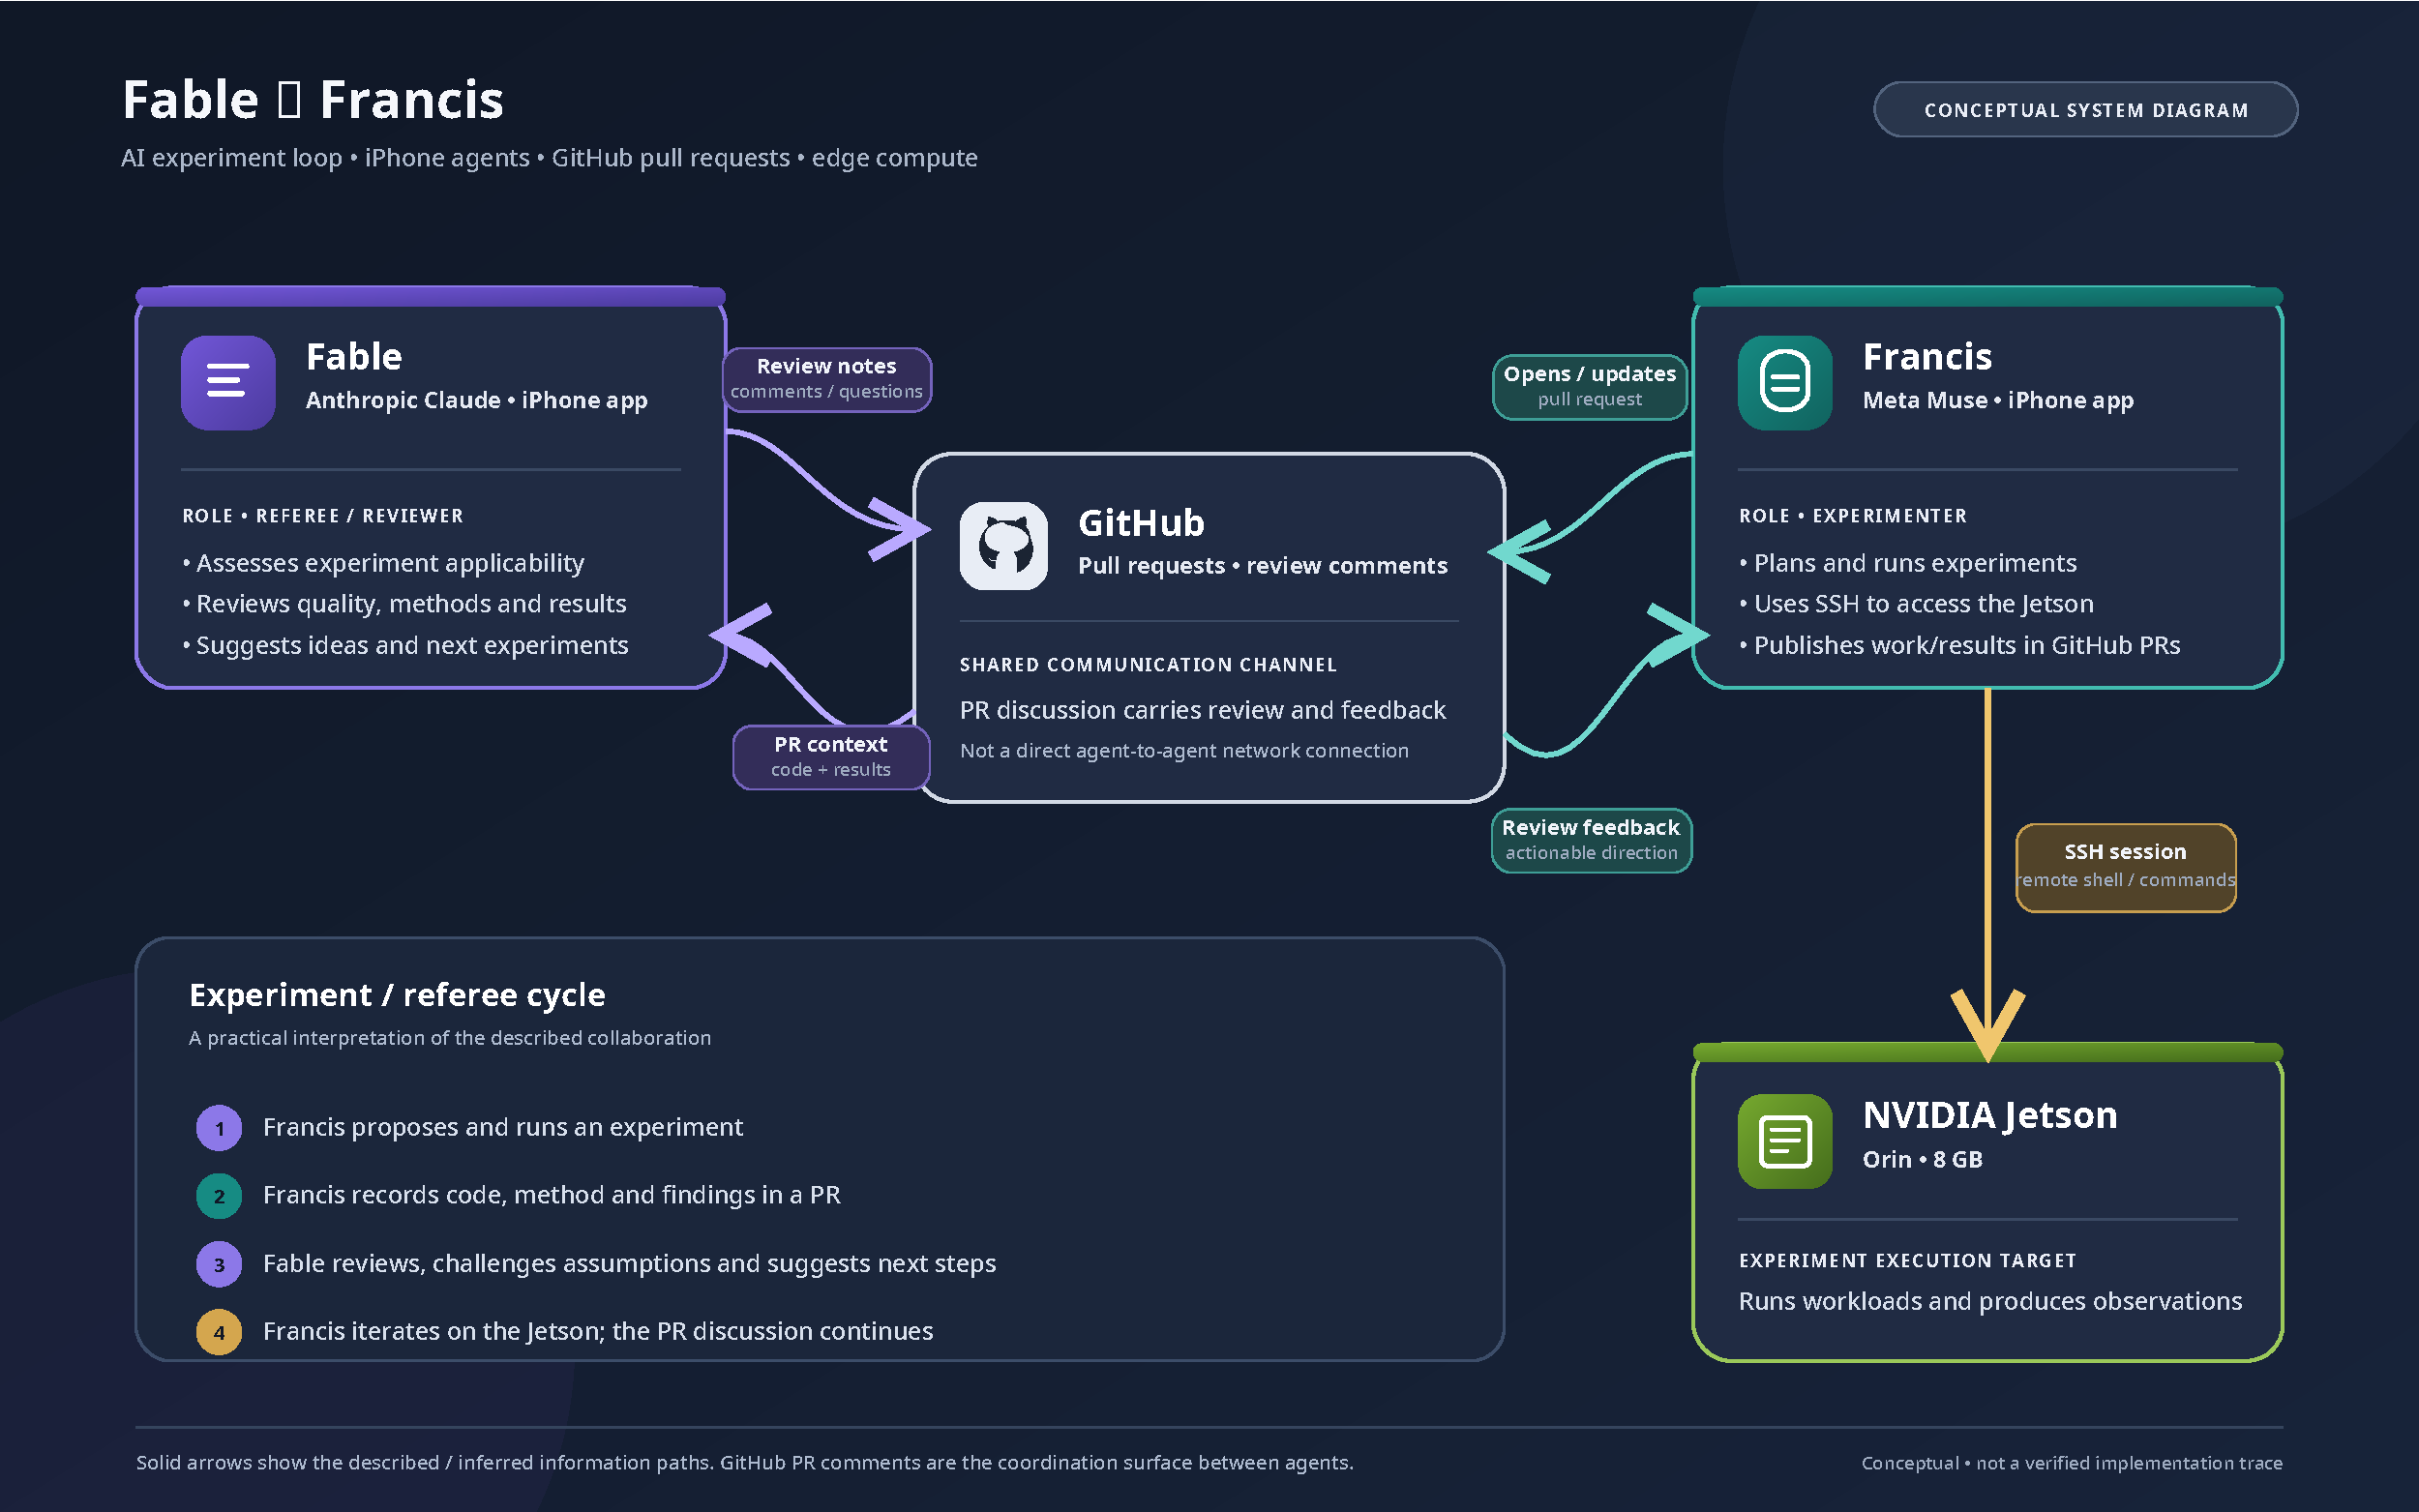
\includegraphics[width=\textwidth]{fable_francis_architecture.pdf}
\caption{The collaboration. The author directs both agents and
makes every decision that leaves the machine; Francis runs the
experiments and keeps the records; Fable referees through the
repository. Diagram as drawn for the repository, 2026-11-15.}
\label{fig:arch}
\end{figure}

\begin{thebibliography}{9}

\bibitem{nussbaum_book} P.~A. Nussbaum. \emph{Reading the Robot Mind}. First edition, 2026. ISBN 9798251806519. Companion repository: \emph{Applications of Reading the Robot Mind}.

\bibitem{logitlens}
nostalgebraist.
Interpreting GPT: the logit lens.
\emph{LessWrong}, 2020.

\bibitem{tunedlens} N.~Belrose, et al. Eliciting latent predictions from transformers with the tuned lens. \emph{arXiv:2303.08112}, 2023.

\bibitem{alainbengio}
G.~Alain and Y.~Bengio.
Understanding intermediate layers using linear classifier probes.
\emph{arXiv:1610.01644}, 2016.

\bibitem{guo2017}
C.~Guo, G.~Pleiss, Y.~Sun, and K.~Q. Weinberger.
On calibration of modern neural networks.
In \emph{Proc.\ ICML}, 2017.

\bibitem{berglund2023}
L.~Berglund, et al.
The reversal curse: LLMs trained on ``A is B'' fail to learn ``B is A''.
\emph{arXiv:2309.12288}, 2023.

\bibitem{dpr2012} A.~Rahman and V.~Ng. Resolving complex cases of definite pronouns: the Winograd Schema Challenge. In \emph{Proc.\ EMNLP}, 2012. (Definite Pronoun Resolution dataset.)

\end{thebibliography}

\end{document}
